\section{Makanya}

\subsection{Hintergrund} % Makanya
Der Hintergrund des Makanya.com Projektes ist eine Partnerschaft zwischen der Kirchengemeinde Kühlungsborn und Tansania,
sowie der Partnerschaft zwischen der Kirchengemeinde und dem Schulzentrum Kühlungsborns.
Der Pastor Kühlungsborns, Matthias Borchert,
suchte den Kontakt zum \jf Team über das Schulzentrum.
% Server: strato.de
% Sprache: Deutsch, Englisch, Zusammenarbeit (Dolmetschering: Frau Wieck)
% Programmierung: PHP, HTML, MySQL
% Beiprogramm: Schulzentrum -> Spendenlauf, Besuch der Tansanianer, Meetings, Auswertung

\subsection{Methodik} % Makanya
% Umgebung: Sublime Text, PHPmyAdmin,
% Hilfe: php.net (erstes PHP Projekt)
% Sicherheit: sha25 Schlüssel, TODO Vortrag herauskramen!
\subsection{Ergebnis} % Makanya
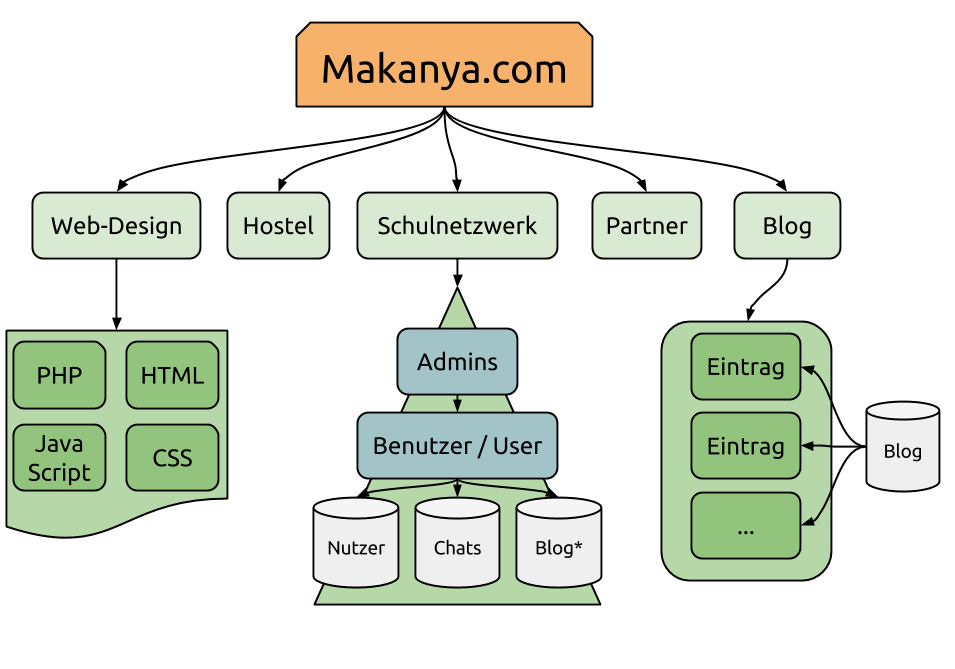
\includegraphics[width=\linewidth]{imgs/makanyaOverview.png}\\
